% =========================================================================
% SECTION 5.8: SIMULATION OF THE SYSTEM (ACTUAL RATING)
% =========================================================================
\section{Simulation of the System (Actual Rating)}

\subsection{Overview of the Simulated System}
In this section, the complete solar-powered EV charging station system is simulated using MATLAB/Simulink under actual component ratings. The purpose of this simulation is to verify that all parts of the system work correctly together as one integrated unit, and to confirm that the power flows properly from the solar panel all the way to both the simulated electric vehicle battery and the energy storage battery.

\begin{figure}[H]
    \centering
    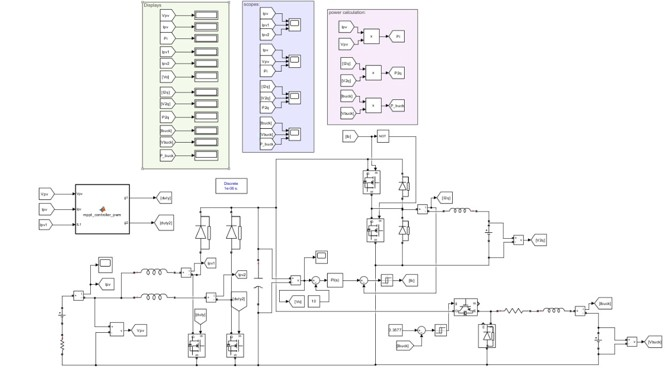
\includegraphics[width=\textwidth]{Figures/1.jpg}
    \caption{Overview of the Simulated System Architecture in Simulink.}
    \label{fig:system_sim_overview}
\end{figure}

The full system consists of five main parts working together:
\begin{itemize}
    \item \textbf{The PV Source:} Represents the solar panel array and provides the primary input power to the system.
    \item \textbf{The MPPT Controller:} Continuously tracks the maximum power point of the solar panel and generates the appropriate duty cycle signals for the input converter phase.
    \item \textbf{The Interleaved Boost Converter:} Takes the PV output voltage and steps it up to a higher DC link voltage of 10~V, which acts as the common intermediate bus for the rest of the system.
    \item \textbf{The Two-Quadrant Chopper:} Takes power from the common DC link and delivers it to the battery storage.
    \item \textbf{The Buck Converter:} Draws power from the DC link and delivers it to the EV battery at a regulated voltage of 3.7~V, utilized when no EV is connected to the charging station.
\end{itemize}

\subsection{PV Source and MPPT Controller Results}
The first scope captures the behavior of the PV side of the system, displaying the PV current ($I_{PV}$), PV voltage ($V_{PV}$), and PV output power ($P_{PV}$) over the simulation timeline.

\begin{figure}[H]
    \centering
    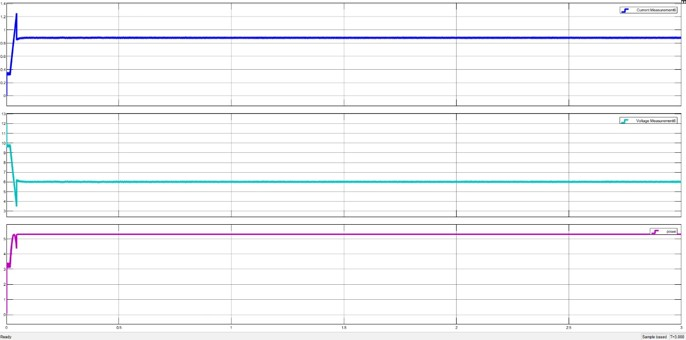
\includegraphics[width=\textwidth]{Figures/2.jpg}
    \caption{PV Side Simulation Results --- $I_{PV}$, $V_{PV}$, and $P_{PV}$.}
    \label{fig:pv_side_results}
\end{figure}

At the start of the simulation, the system goes through a brief startup transient. The PV current starts from zero and rises quickly, reaching a peak of approximately 1.4~A before settling down. At the same time, the PV voltage starts at a higher value of around 12~V and drops sharply as the MPPT controller begins adjusting the duty cycle to push the operating point toward the maximum power point. Within approximately 0.1 seconds, both the current and voltage settle to their final steady-state values.

After the transient period, the system reaches a stable operating point where:
\begin{itemize}
    \item PV Voltage ($V_{PV}$) = 6.051~V
    \item PV Current ($I_{PV}$) = 0.8749~A
    \item PV Output Power ($P_{PV}$) = 5.294~W
\end{itemize}

These values confirm that the MPPT controller has successfully driven the operating point of the solar panel to its maximum power point. This can be verified by the simple calculation:
\begin{equation}
    V_{PV} \times I_{PV} = 6.051 \times 0.8749 \approx 5.294\text{ W}
\end{equation}
which exactly matches the power value shown in the display. After this point, all three signals remain flat and stable for the rest of the simulation, with only a very small ripple visible on the current and power waveforms. This small ripple is a normal result of the high-frequency switching action of the interleaved boost converter and does not affect the overall system performance. The fast settling and stable behavior of the MPPT controller demonstrate that the control algorithm is working correctly and that the system is able to extract the maximum available power from the solar panel under the given operating conditions.

\subsection{Interleaved Boost Converter Results}
The interleaved boost converter is the heart of the system on the generation side. Unlike a conventional single-phase boost converter, the interleaved boost converter used in this project has two parallel phases, each consisting of its own inductor and switching MOSFET. The two phases are controlled with the same switching frequency but with a 180$^\circ$ phase shift between them. 

This interleaving technique provides two important advantages: it reduces the current ripple seen by the PV source, and it distributes the total current between two inductors instead of one, which reduces stress on each individual component. The scope for the interleaved boost converter shows three current signals: the total PV current ($I_{PV}$ in red), the current through inductor 1 ($I_{PV1}$ in blue), and the current through inductor 2 ($I_{PV2}$ in orange).

\begin{figure}[H]
    \centering
    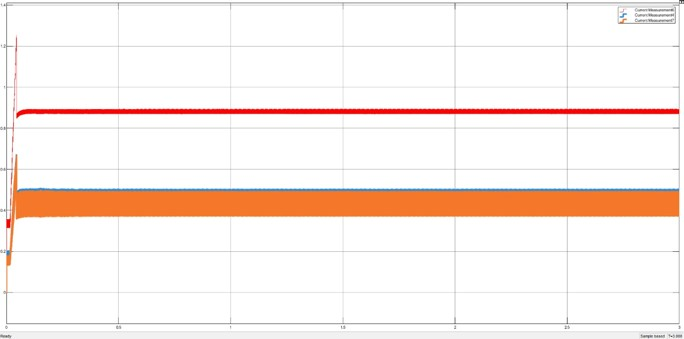
\includegraphics[width=\textwidth]{Figures/3.jpg}
    \caption{Interleaved Boost Converter Current Profiles --- $I_{PV}$, $I_{PV1}$, $I_{PV2}$ (Full View).}
    \label{fig:interleaved_full_view}
\end{figure}

\begin{figure}[H]
    \centering
    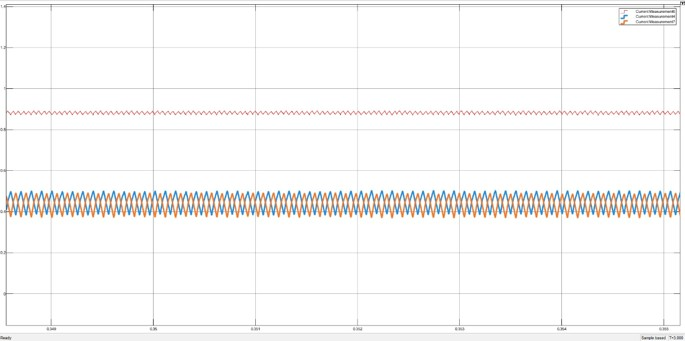
\includegraphics[width=\textwidth]{Figures/4.jpg}
    \caption{Interleaved Boost Converter Current Profiles --- $I_{PV}$, $I_{PV1}$, $I_{PV2}$ (Zoomed View showing 180$^\circ$ interleaving waveforms).}
    \label{fig:interleaved_zoomed_view}
\end{figure}

Looking at the full simulation view, the total PV current (red) settles to approximately 0.8749~A after the startup transient, which is consistent with the MPPT operating point discussed in the previous section. The two individual inductor currents settle to:
\begin{itemize}
    \item $I_{PV1}$ = 0.3903~A
    \item $I_{PV2}$ = 0.4846~A
\end{itemize}

It can be verified that $I_{PV1} + I_{PV2} = 0.3903 + 0.4846 = 0.8749$A,
which is exactly equal to the total PV current. This confirms that the total current from the PV source is correctly shared between the two phases of the interleaved boost converter, with each phase carrying approximately half of the total current. 

The zoomed view of the same scope reveals the detailed waveform shapes of the three currents at steady state. The two inductor currents ($I_{PV1}$ in blue and $I_{PV2}$ in orange) show clear triangular waveforms, which is the expected shape for inductor current in a switching converter. The current rises linearly when the switch is ON as the inductor stores energy, and falls linearly when the switch is OFF as the inductor releases energy to the output. 

Most importantly, the two triangular waveforms are clearly \textbf{180$^\circ$ out of phase} with each other, which confirms that the interleaving is working correctly. Because the two-phase currents are phase-shifted by 180$^\circ$, their ripple components partially cancel each other when they are combined into the total PV current. As a result, the total current (red) has a noticeably smaller ripple amplitude and a higher ripple frequency compared to either individual phase current. This ripple cancellation is one of the main reasons for choosing the interleaved topology in this project, as it reduces the stress on the PV source and improves the overall quality of the current drawn from the solar panel.
\newpage
The DC link voltage was regulated by the interleaved boost converter to a reference value of $V_{out} = 10$~V, as confirmed by the display block output. This 10~V DC link serves as the common intermediate bus from which both the two-quadrant chopper and the buck converter draw their input power.

\subsection{Two-Quadrant Chopper Results (EV Battery Charging)}
The two-quadrant chopper is responsible for delivering power from the 10~V DC link to the simulated electric vehicle battery. The EV battery is represented in this simulation by a 2S IMR14500 lithium-ion battery pack with a nominal voltage of 7.4~V. The scope for this stage shows the output current ($I_{2Q}$), output voltage ($V_{2Q}$), and output power ($P_{2Q}$).

\begin{figure}[H]
    \centering
    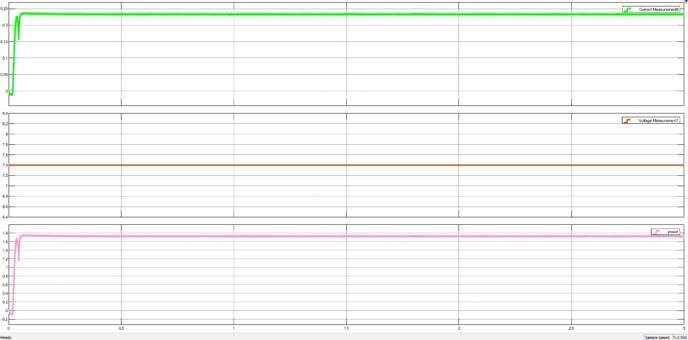
\includegraphics[width=\textwidth]{Figures/5.jpg}
    \caption{Two-Quadrant Chopper Results --- $I_{2Q}$, $V_{2Q}$, and $P_{2Q}$.}
    \label{fig:two_quad_chopper_results}
\end{figure}

At the start of the simulation, both the current and power start from zero and rise smoothly toward their final values. A small overshoot is visible during the startup transient, after which both signals settle quickly and cleanly to their steady-state values within approximately 0.1 seconds. The output voltage ($V_{2Q}$), on the other hand, shows no transient at all --- it is immediately stable at 7.4~V from the very beginning of the simulation, which reflects the voltage regulation behavior of the chopper's control loop.

After the transient period, the three output signals reach the following steady-state values:
\begin{itemize}
    \item Output Current ($I_{2Q}$) = 0.2319~A
    \item Output Voltage ($V_{2Q}$) = 7.4~V
    \item Output Power ($P_{2Q}$) = 1.716~W
\end{itemize}

These values can be cross-checked analytically:
\begin{equation}
    V_{2Q} \times I_{2Q} = 7.4 \times 0.2319 \approx 1.716\text{ W}
\end{equation}
The steady-state output voltage of 7.4~V is exactly equal to the nominal voltage of the simulated EV battery pack, which confirms that the two-quadrant chopper is correctly stepping down the 10~V DC link voltage to the level required to charge the EV battery. All three signals remain perfectly flat and stable for the remaining 2.9 seconds of the simulation, with no visible ripple or disturbance, confirming stable and reliable operation of this stage.

\subsection{Buck Converter Results (EV Battery Charging)}
The buck converter is responsible for delivering power from the 10~V DC link to the energy storage battery, which is used when no electric vehicle is connected to the charging station. Like the two-quadrant chopper output, the storage battery also has a nominal voltage of 7.4~V (2S ICR18650 pack). The scope for this stage shows the output current ($I_{buck}$), output voltage ($V_{buck}$), and output power ($P_{buck}$).

\begin{figure}[H]
    \centering
    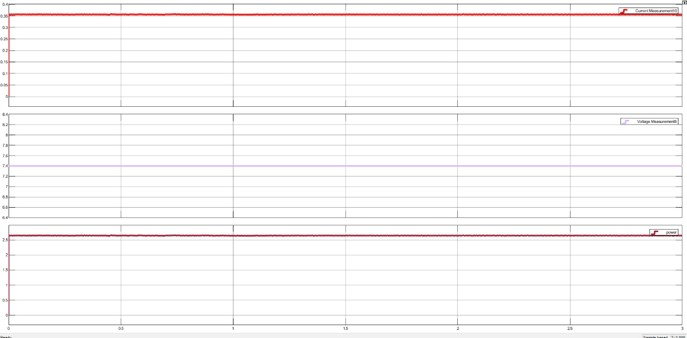
\includegraphics[width=\textwidth]{Figures/6.jpg}
    \caption{Buck Converter Results --- $I_{buck}$, $V_{buck}$, and $P_{buck}$.}
    \label{fig:buck_converter_results}
\end{figure}

Unlike the two-quadrant chopper, the buck converter scope shows no startup transient at all --- all three signals are immediately at their steady-state values from the very first moment of the simulation ($t = 0$). This is because the buck converter's control loop reaches its operating point almost instantaneously under the given initial conditions.

The three signals show a small but visible high-frequency ripple throughout the entire simulation. This ripple is a normal characteristic of a buck converter operating in continuous conduction mode and is caused by the switching action of the MOSFET. The ripple amplitude is small relative to the average values, confirming that the converter's passive components (inductor and output capacitor) are appropriately sized to keep the output ripple within acceptable limits.

\pagebreak % Clean alignment split before final results matrix

The steady-state values of the buck converter output are:
\begin{itemize}
    \item Output Current ($I_{buck}$) = 0.3559~A
    \item Output Voltage ($V_{buck}$) = 7.4~V
    \item Output Power ($P_{buck}$) = 2.634~W
\end{itemize}

Again, these values can be verified analytically:
\begin{equation}
    V_{buck} \times I_{buck} = 7.4 \times 0.3559 \approx 2.634\text{ W}
\end{equation}
The output voltage is regulated to exactly 7.4~V, matching the nominal voltage of the storage battery, which confirms that the buck converter is correctly charging the storage battery at the right voltage level. The fact that the output voltage is stable and well-regulated throughout the simulation confirms that the buck converter's control loop is functioning correctly.
\newpage
\subsection{Summary of Simulation Results}
The tracking performance and electrical measurements extracted across the integrated system are summarized in Table 5.2.

\begin{table}[H]
    \centering
    \caption{Comprehensive Full-System Simulation Results Matrix}
    \label{tab:system_simulation_summary}
    \noindent
    \centerline{% Forces table width containment to prevent margin overflow loops
    \begin{tabularx}{\textwidth}{>{\bfseries\raggedright\arraybackslash}X c}
        \toprule
        Parameter Description & Simulated Steady-State Value \\
        \midrule
        PV Source Voltage ($V_{PV}$) & 6.051 V \\
        PV Source Current ($I_{PV}$) & 0.8749 A \\
        PV Source Output Power ($P_{PV}$) & 5.294 W \\
        \midrule
        Interleaved Boost Inductor 1 Current ($I_{PV1}$) & 0.3903 A \\
        Interleaved Boost Inductor 2 Current ($I_{PV2}$) & 0.4846 A \\
        Intermediate DC Link Bus Voltage ($V_{out}$) & 10.000 V \\
        \midrule
        Two-Quadrant Chopper Output Voltage ($V_{2Q}$) & 7.400 V \\
        Two-Quadrant Chopper Output Current ($I_{2Q}$) & 0.2319 A \\
        Two-Quadrant Chopper Output Power ($P_{2Q}$) & 1.716 W \\
        \midrule
        Auxiliary Buck Converter Output Voltage ($V_{Buck}$) & 7.400 V \\
        Auxiliary Buck Converter Output Current ($I_{Buck}$) & 0.3559 A \\
        Auxiliary Buck Converter Output Power ($P_{Buck}$) & 2.634 W \\
        \bottomrule
    \end{tabularx}%
    }
\end{table}

The full simulation results confirm that the complete PV-based EV charging station system operates correctly as an integrated unit. The MPPT controller successfully extracts the maximum available power from the solar panel, the interleaved boost converter steps up the PV voltage to the 10~V DC link with reduced current ripple due to the interleaving effect, and both the two-quadrant chopper and buck converter successfully regulate their output voltages to 7.4~V to charge the simulated EV battery and the storage battery respectively. All signals reach stable steady-state values quickly and remain stable throughout the simulation, confirming the effectiveness of the overall system design and control strategy.